% Created by tikzDevice version 0.6.2-92-0ad2792 on 2013-01-13 15:13:08
% !TEX encoding = UTF-8 Unicode
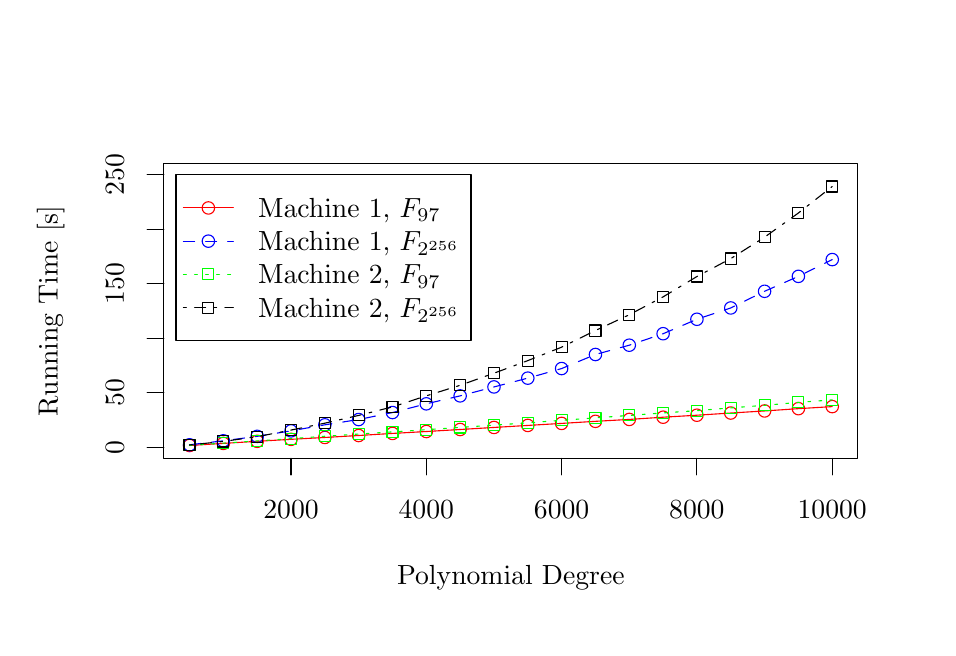
\begin{tikzpicture}[x=1pt,y=1pt]
\definecolor[named]{fillColor}{rgb}{1.00,1.00,1.00}
\path[use as bounding box,fill=fillColor,fill opacity=0.00] (0,0) rectangle (325.21,216.81);
\begin{scope}
\path[clip] ( 49.20, 61.20) rectangle (300.01,167.61);
\definecolor[named]{drawColor}{rgb}{1.00,0.00,0.00}

\path[draw=drawColor,line width= 0.4pt,line join=round,line cap=round] ( 58.49, 65.83) --
	( 70.71, 66.59) --
	( 82.94, 67.34) --
	( 95.16, 68.06) --
	(107.38, 68.73) --
	(119.60, 69.44) --
	(131.83, 70.19) --
	(144.05, 70.88) --
	(156.27, 71.61) --
	(168.50, 72.35) --
	(180.72, 73.08) --
	(192.94, 73.81) --
	(205.16, 74.56) --
	(217.39, 75.25) --
	(229.61, 76.05) --
	(241.83, 76.77) --
	(254.06, 77.56) --
	(266.28, 78.31) --
	(278.50, 79.14) --
	(290.73, 79.88);

\path[draw=drawColor,line width= 0.4pt,line join=round,line cap=round] ( 58.49, 65.83) circle (  2.25);

\path[draw=drawColor,line width= 0.4pt,line join=round,line cap=round] ( 70.71, 66.59) circle (  2.25);

\path[draw=drawColor,line width= 0.4pt,line join=round,line cap=round] ( 82.94, 67.34) circle (  2.25);

\path[draw=drawColor,line width= 0.4pt,line join=round,line cap=round] ( 95.16, 68.06) circle (  2.25);

\path[draw=drawColor,line width= 0.4pt,line join=round,line cap=round] (107.38, 68.73) circle (  2.25);

\path[draw=drawColor,line width= 0.4pt,line join=round,line cap=round] (119.60, 69.44) circle (  2.25);

\path[draw=drawColor,line width= 0.4pt,line join=round,line cap=round] (131.83, 70.19) circle (  2.25);

\path[draw=drawColor,line width= 0.4pt,line join=round,line cap=round] (144.05, 70.88) circle (  2.25);

\path[draw=drawColor,line width= 0.4pt,line join=round,line cap=round] (156.27, 71.61) circle (  2.25);

\path[draw=drawColor,line width= 0.4pt,line join=round,line cap=round] (168.50, 72.35) circle (  2.25);

\path[draw=drawColor,line width= 0.4pt,line join=round,line cap=round] (180.72, 73.08) circle (  2.25);

\path[draw=drawColor,line width= 0.4pt,line join=round,line cap=round] (192.94, 73.81) circle (  2.25);

\path[draw=drawColor,line width= 0.4pt,line join=round,line cap=round] (205.16, 74.56) circle (  2.25);

\path[draw=drawColor,line width= 0.4pt,line join=round,line cap=round] (217.39, 75.25) circle (  2.25);

\path[draw=drawColor,line width= 0.4pt,line join=round,line cap=round] (229.61, 76.05) circle (  2.25);

\path[draw=drawColor,line width= 0.4pt,line join=round,line cap=round] (241.83, 76.77) circle (  2.25);

\path[draw=drawColor,line width= 0.4pt,line join=round,line cap=round] (254.06, 77.56) circle (  2.25);

\path[draw=drawColor,line width= 0.4pt,line join=round,line cap=round] (266.28, 78.31) circle (  2.25);

\path[draw=drawColor,line width= 0.4pt,line join=round,line cap=round] (278.50, 79.14) circle (  2.25);

\path[draw=drawColor,line width= 0.4pt,line join=round,line cap=round] (290.73, 79.88) circle (  2.25);
\end{scope}
\begin{scope}
\path[clip] (  0.00,  0.00) rectangle (325.21,216.81);
\definecolor[named]{drawColor}{rgb}{0.00,0.00,0.00}

\path[draw=drawColor,line width= 0.4pt,line join=round,line cap=round] ( 95.16, 61.20) -- (290.73, 61.20);

\path[draw=drawColor,line width= 0.4pt,line join=round,line cap=round] ( 95.16, 61.20) -- ( 95.16, 55.20);

\path[draw=drawColor,line width= 0.4pt,line join=round,line cap=round] (144.05, 61.20) -- (144.05, 55.20);

\path[draw=drawColor,line width= 0.4pt,line join=round,line cap=round] (192.94, 61.20) -- (192.94, 55.20);

\path[draw=drawColor,line width= 0.4pt,line join=round,line cap=round] (241.83, 61.20) -- (241.83, 55.20);

\path[draw=drawColor,line width= 0.4pt,line join=round,line cap=round] (290.73, 61.20) -- (290.73, 55.20);

\node[text=drawColor,anchor=base,inner sep=0pt, outer sep=0pt, scale=  1.00] at ( 95.16, 39.60) {2000};

\node[text=drawColor,anchor=base,inner sep=0pt, outer sep=0pt, scale=  1.00] at (144.05, 39.60) {4000};

\node[text=drawColor,anchor=base,inner sep=0pt, outer sep=0pt, scale=  1.00] at (192.94, 39.60) {6000};

\node[text=drawColor,anchor=base,inner sep=0pt, outer sep=0pt, scale=  1.00] at (241.83, 39.60) {8000};

\node[text=drawColor,anchor=base,inner sep=0pt, outer sep=0pt, scale=  1.00] at (290.73, 39.60) {10000};

\path[draw=drawColor,line width= 0.4pt,line join=round,line cap=round] ( 49.20, 65.14) -- ( 49.20,163.67);

\path[draw=drawColor,line width= 0.4pt,line join=round,line cap=round] ( 49.20, 65.14) -- ( 43.20, 65.14);

\path[draw=drawColor,line width= 0.4pt,line join=round,line cap=round] ( 49.20, 84.85) -- ( 43.20, 84.85);

\path[draw=drawColor,line width= 0.4pt,line join=round,line cap=round] ( 49.20,104.55) -- ( 43.20,104.55);

\path[draw=drawColor,line width= 0.4pt,line join=round,line cap=round] ( 49.20,124.26) -- ( 43.20,124.26);

\path[draw=drawColor,line width= 0.4pt,line join=round,line cap=round] ( 49.20,143.96) -- ( 43.20,143.96);

\path[draw=drawColor,line width= 0.4pt,line join=round,line cap=round] ( 49.20,163.67) -- ( 43.20,163.67);

\node[text=drawColor,rotate= 90.00,anchor=base,inner sep=0pt, outer sep=0pt, scale=  1.00] at ( 34.80, 65.14) {0};

\node[text=drawColor,rotate= 90.00,anchor=base,inner sep=0pt, outer sep=0pt, scale=  1.00] at ( 34.80, 84.85) {50};

\node[text=drawColor,rotate= 90.00,anchor=base,inner sep=0pt, outer sep=0pt, scale=  1.00] at ( 34.80,124.26) {150};

\node[text=drawColor,rotate= 90.00,anchor=base,inner sep=0pt, outer sep=0pt, scale=  1.00] at ( 34.80,163.67) {250};

\path[draw=drawColor,line width= 0.4pt,line join=round,line cap=round] ( 49.20, 61.20) --
	(300.01, 61.20) --
	(300.01,167.61) --
	( 49.20,167.61) --
	( 49.20, 61.20);
\end{scope}
\begin{scope}
\path[clip] (  0.00,  0.00) rectangle (325.21,216.81);
\definecolor[named]{drawColor}{rgb}{0.00,0.00,0.00}

\node[text=drawColor,anchor=base,inner sep=0pt, outer sep=0pt, scale=  1.00] at (174.61, 15.60) {Polynomial Degree};

\node[text=drawColor,rotate= 90.00,anchor=base,inner sep=0pt, outer sep=0pt, scale=  1.00] at ( 10.80,114.41) {Running Time [s]};
\end{scope}
\begin{scope}
\path[clip] ( 49.20, 61.20) rectangle (300.01,167.61);
\definecolor[named]{drawColor}{rgb}{0.00,0.00,1.00}

\path[draw=drawColor,line width= 0.4pt,dash pattern=on 4pt off 4pt ,line join=round,line cap=round] ( 58.49, 66.08) --
	( 70.71, 67.52) --
	( 82.94, 69.14) --
	( 95.16, 71.12) --
	(107.38, 73.30) --
	(119.60, 75.21) --
	(131.83, 77.74) --
	(144.05, 80.88) --
	(156.27, 83.76) --
	(168.50, 86.99) --
	(180.72, 90.17) --
	(192.94, 93.63) --
	(205.16, 98.71) --
	(217.39,102.07) --
	(229.61,106.22) --
	(241.83,111.44) --
	(254.06,115.53) --
	(266.28,121.55) --
	(278.50,126.95) --
	(290.73,133.01);

\path[draw=drawColor,line width= 0.4pt,line join=round,line cap=round] ( 58.49, 66.08) circle (  2.25);

\path[draw=drawColor,line width= 0.4pt,line join=round,line cap=round] ( 70.71, 67.52) circle (  2.25);

\path[draw=drawColor,line width= 0.4pt,line join=round,line cap=round] ( 82.94, 69.14) circle (  2.25);

\path[draw=drawColor,line width= 0.4pt,line join=round,line cap=round] ( 95.16, 71.12) circle (  2.25);

\path[draw=drawColor,line width= 0.4pt,line join=round,line cap=round] (107.38, 73.30) circle (  2.25);

\path[draw=drawColor,line width= 0.4pt,line join=round,line cap=round] (119.60, 75.21) circle (  2.25);

\path[draw=drawColor,line width= 0.4pt,line join=round,line cap=round] (131.83, 77.74) circle (  2.25);

\path[draw=drawColor,line width= 0.4pt,line join=round,line cap=round] (144.05, 80.88) circle (  2.25);

\path[draw=drawColor,line width= 0.4pt,line join=round,line cap=round] (156.27, 83.76) circle (  2.25);

\path[draw=drawColor,line width= 0.4pt,line join=round,line cap=round] (168.50, 86.99) circle (  2.25);

\path[draw=drawColor,line width= 0.4pt,line join=round,line cap=round] (180.72, 90.17) circle (  2.25);

\path[draw=drawColor,line width= 0.4pt,line join=round,line cap=round] (192.94, 93.63) circle (  2.25);

\path[draw=drawColor,line width= 0.4pt,line join=round,line cap=round] (205.16, 98.71) circle (  2.25);

\path[draw=drawColor,line width= 0.4pt,line join=round,line cap=round] (217.39,102.07) circle (  2.25);

\path[draw=drawColor,line width= 0.4pt,line join=round,line cap=round] (229.61,106.22) circle (  2.25);

\path[draw=drawColor,line width= 0.4pt,line join=round,line cap=round] (241.83,111.44) circle (  2.25);

\path[draw=drawColor,line width= 0.4pt,line join=round,line cap=round] (254.06,115.53) circle (  2.25);

\path[draw=drawColor,line width= 0.4pt,line join=round,line cap=round] (266.28,121.55) circle (  2.25);

\path[draw=drawColor,line width= 0.4pt,line join=round,line cap=round] (278.50,126.95) circle (  2.25);

\path[draw=drawColor,line width= 0.4pt,line join=round,line cap=round] (290.73,133.01) circle (  2.25);
\definecolor[named]{drawColor}{rgb}{0.00,1.00,0.00}

\path[draw=drawColor,line width= 0.4pt,dash pattern=on 1pt off 3pt ,line join=round,line cap=round] ( 58.49, 65.90) --
	( 70.71, 66.68) --
	( 82.94, 67.49) --
	( 95.16, 68.32) --
	(107.38, 69.16) --
	(119.60, 69.96) --
	(131.83, 70.74) --
	(144.05, 71.54) --
	(156.27, 72.36) --
	(168.50, 73.19) --
	(180.72, 74.01) --
	(192.94, 74.93) --
	(205.16, 75.81) --
	(217.39, 76.69) --
	(229.61, 77.60) --
	(241.83, 78.42) --
	(254.06, 79.42) --
	(266.28, 80.35) --
	(278.50, 81.40) --
	(290.73, 82.31);

\path[draw=drawColor,line width= 0.4pt,line join=round,line cap=round] ( 56.50, 63.90) rectangle ( 60.48, 67.89);

\path[draw=drawColor,line width= 0.4pt,line join=round,line cap=round] ( 68.72, 64.69) rectangle ( 72.71, 68.67);

\path[draw=drawColor,line width= 0.4pt,line join=round,line cap=round] ( 80.94, 65.50) rectangle ( 84.93, 69.48);

\path[draw=drawColor,line width= 0.4pt,line join=round,line cap=round] ( 93.16, 66.32) rectangle ( 97.15, 70.31);

\path[draw=drawColor,line width= 0.4pt,line join=round,line cap=round] (105.39, 67.17) rectangle (109.38, 71.15);

\path[draw=drawColor,line width= 0.4pt,line join=round,line cap=round] (117.61, 67.96) rectangle (121.60, 71.95);

\path[draw=drawColor,line width= 0.4pt,line join=round,line cap=round] (129.83, 68.74) rectangle (133.82, 72.73);

\path[draw=drawColor,line width= 0.4pt,line join=round,line cap=round] (142.06, 69.55) rectangle (146.04, 73.54);

\path[draw=drawColor,line width= 0.4pt,line join=round,line cap=round] (154.28, 70.36) rectangle (158.27, 74.35);

\path[draw=drawColor,line width= 0.4pt,line join=round,line cap=round] (166.50, 71.19) rectangle (170.49, 75.18);

\path[draw=drawColor,line width= 0.4pt,line join=round,line cap=round] (178.72, 72.01) rectangle (182.71, 76.00);

\path[draw=drawColor,line width= 0.4pt,line join=round,line cap=round] (190.95, 72.93) rectangle (194.94, 76.92);

\path[draw=drawColor,line width= 0.4pt,line join=round,line cap=round] (203.17, 73.82) rectangle (207.16, 77.81);

\path[draw=drawColor,line width= 0.4pt,line join=round,line cap=round] (215.39, 74.70) rectangle (219.38, 78.69);

\path[draw=drawColor,line width= 0.4pt,line join=round,line cap=round] (227.62, 75.60) rectangle (231.60, 79.59);

\path[draw=drawColor,line width= 0.4pt,line join=round,line cap=round] (239.84, 76.43) rectangle (243.83, 80.41);

\path[draw=drawColor,line width= 0.4pt,line join=round,line cap=round] (252.06, 77.43) rectangle (256.05, 81.41);

\path[draw=drawColor,line width= 0.4pt,line join=round,line cap=round] (264.29, 78.35) rectangle (268.27, 82.34);

\path[draw=drawColor,line width= 0.4pt,line join=round,line cap=round] (276.51, 79.40) rectangle (280.50, 83.39);

\path[draw=drawColor,line width= 0.4pt,line join=round,line cap=round] (288.73, 80.31) rectangle (292.72, 84.30);
\definecolor[named]{drawColor}{rgb}{0.00,0.00,0.00}

\path[draw=drawColor,line width= 0.4pt,dash pattern=on 1pt off 3pt on 4pt off 3pt ,line join=round,line cap=round] ( 58.49, 66.01) --
	( 70.71, 67.30) --
	( 82.94, 69.01) --
	( 95.16, 71.41) --
	(107.38, 73.89) --
	(119.60, 76.70) --
	(131.83, 79.77) --
	(144.05, 83.77) --
	(156.27, 87.59) --
	(168.50, 91.95) --
	(180.72, 96.50) --
	(192.94,101.36) --
	(205.16,107.37) --
	(217.39,113.08) --
	(229.61,119.54) --
	(241.83,126.88) --
	(254.06,133.37) --
	(266.28,141.10) --
	(278.50,149.84) --
	(290.73,159.42);

\path[draw=drawColor,line width= 0.4pt,line join=round,line cap=round] ( 56.50, 64.01) rectangle ( 60.48, 68.00);

\path[draw=drawColor,line width= 0.4pt,line join=round,line cap=round] ( 68.72, 65.30) rectangle ( 72.71, 69.29);

\path[draw=drawColor,line width= 0.4pt,line join=round,line cap=round] ( 80.94, 67.02) rectangle ( 84.93, 71.01);

\path[draw=drawColor,line width= 0.4pt,line join=round,line cap=round] ( 93.16, 69.42) rectangle ( 97.15, 73.40);

\path[draw=drawColor,line width= 0.4pt,line join=round,line cap=round] (105.39, 71.90) rectangle (109.38, 75.89);

\path[draw=drawColor,line width= 0.4pt,line join=round,line cap=round] (117.61, 74.71) rectangle (121.60, 78.70);

\path[draw=drawColor,line width= 0.4pt,line join=round,line cap=round] (129.83, 77.77) rectangle (133.82, 81.76);

\path[draw=drawColor,line width= 0.4pt,line join=round,line cap=round] (142.06, 81.78) rectangle (146.04, 85.77);

\path[draw=drawColor,line width= 0.4pt,line join=round,line cap=round] (154.28, 85.60) rectangle (158.27, 89.59);

\path[draw=drawColor,line width= 0.4pt,line join=round,line cap=round] (166.50, 89.96) rectangle (170.49, 93.94);

\path[draw=drawColor,line width= 0.4pt,line join=round,line cap=round] (178.72, 94.51) rectangle (182.71, 98.50);

\path[draw=drawColor,line width= 0.4pt,line join=round,line cap=round] (190.95, 99.36) rectangle (194.94,103.35);

\path[draw=drawColor,line width= 0.4pt,line join=round,line cap=round] (203.17,105.37) rectangle (207.16,109.36);

\path[draw=drawColor,line width= 0.4pt,line join=round,line cap=round] (215.39,111.08) rectangle (219.38,115.07);

\path[draw=drawColor,line width= 0.4pt,line join=round,line cap=round] (227.62,117.55) rectangle (231.60,121.54);

\path[draw=drawColor,line width= 0.4pt,line join=round,line cap=round] (239.84,124.89) rectangle (243.83,128.87);

\path[draw=drawColor,line width= 0.4pt,line join=round,line cap=round] (252.06,131.38) rectangle (256.05,135.37);

\path[draw=drawColor,line width= 0.4pt,line join=round,line cap=round] (264.29,139.11) rectangle (268.27,143.10);

\path[draw=drawColor,line width= 0.4pt,line join=round,line cap=round] (276.51,147.85) rectangle (280.50,151.83);

\path[draw=drawColor,line width= 0.4pt,line join=round,line cap=round] (288.73,157.43) rectangle (292.72,161.41);

\path[draw=drawColor,line width= 0.4pt,line join=round,line cap=round] ( 53.60,163.67) rectangle (160.20,103.67);
\definecolor[named]{drawColor}{rgb}{1.00,0.00,0.00}

\path[draw=drawColor,line width= 0.4pt,line join=round,line cap=round] ( 56.30,151.67) -- ( 74.30,151.67);
\definecolor[named]{drawColor}{rgb}{0.00,0.00,1.00}

\path[draw=drawColor,line width= 0.4pt,dash pattern=on 4pt off 4pt ,line join=round,line cap=round] ( 56.30,139.67) -- ( 74.30,139.67);
\definecolor[named]{drawColor}{rgb}{0.00,1.00,0.00}

\path[draw=drawColor,line width= 0.4pt,dash pattern=on 1pt off 3pt ,line join=round,line cap=round] ( 56.30,127.67) -- ( 74.30,127.67);
\definecolor[named]{drawColor}{rgb}{0.00,0.00,0.00}

\path[draw=drawColor,line width= 0.4pt,dash pattern=on 1pt off 3pt on 4pt off 3pt ,line join=round,line cap=round] ( 56.30,115.67) -- ( 74.30,115.67);
\definecolor[named]{drawColor}{rgb}{1.00,0.00,0.00}

\path[draw=drawColor,line width= 0.4pt,line join=round,line cap=round] ( 65.30,151.67) circle (  2.25);
\definecolor[named]{drawColor}{rgb}{0.00,0.00,1.00}

\path[draw=drawColor,line width= 0.4pt,line join=round,line cap=round] ( 65.30,139.67) circle (  2.25);
\definecolor[named]{drawColor}{rgb}{0.00,1.00,0.00}

\path[draw=drawColor,line width= 0.4pt,line join=round,line cap=round] ( 63.31,125.67) rectangle ( 67.29,129.66);
\definecolor[named]{drawColor}{rgb}{0.00,0.00,0.00}

\path[draw=drawColor,line width= 0.4pt,line join=round,line cap=round] ( 63.31,113.67) rectangle ( 67.29,117.66);

\node[text=drawColor,anchor=base west,inner sep=0pt, outer sep=0pt, scale=  1.00] at ( 83.30,148.23) {Machine 1, $\mathbb{F}_{97}$};

\node[text=drawColor,anchor=base west,inner sep=0pt, outer sep=0pt, scale=  1.00] at ( 83.30,136.23) {Machine 1, $\mathbb{F}_{2^{256}}$};

\node[text=drawColor,anchor=base west,inner sep=0pt, outer sep=0pt, scale=  1.00] at ( 83.30,124.23) {Machine 2, $\mathbb{F}_{97}$};

\node[text=drawColor,anchor=base west,inner sep=0pt, outer sep=0pt, scale=  1.00] at ( 83.30,112.23) {Machine 2, $\mathbb{F}_{2^{256}}$};
\end{scope}
\end{tikzpicture}
